%%% template.tex
%%%
%%% This LaTeX source document can be used as the basis for your technical
%%% paper or abstract.

%%% The parameter to the ``documentclass'' command is very important.
%%% - use ``review'' for content submitted for review.
%%% - use ``preprint'' for accepted content you are making available.
%%% - use ``tog'' for technical papers accepted to the TOG journal and
%%%   for presentation at the SIGGRAPH or SIGGRAPH Asia conference.
%%% - use ``conference'' for final content accepted to a sponsored event
%%%   (hint: If you don't know, you should use ``conference.'')
\documentclass[tog]{acmsiggraph}

%%% Make the ``BibTeX'' word pretty...

\def\BibTeX{{\rm B\kern-.05em{\sc i\kern-.025em b}\kern-.08em
    T\kern-.1667em\lower.7ex\hbox{E}\kern-.125emX}}

%%% Used by the ``review'' variation; the online ID will be printed on 
%%% every page of the content.

\TOGonlineid{45678}

%%% Used by the ``preprint'' variation.

\TOGvolume{0}
\TOGnumber{0}

\title{Real-time Aerodynamic Sound Synthesis for Slender Objects }

\author{Jui-Hsien Wang\thanks{e-mail:jw969@cornell.edu}\\Cornell University}
\pdfauthor{Jui-Hsien Wang}

\keywords{}


\usepackage{color}
\usepackage{url}

% symbol definition
\def\p{\partial} 
\def\f{\frac} 
\def\n{\nabla} 
\def\t{\tilde}
\def\mb{\mathbf} 
\def\tb{\textbf} 
\def\etal{\emph{et al.}}
\def\tss{\textsuperscript}

\def\mbxt{(\mb{x},t)}
\def\mbtxt{(\mb{\t{x}},t)}

%%%%%%%%%%%%%%%%%%%%%%%%%%%%%%%%%%%%%%%%%
\begin{document}

%%% This is the ``teaser'' command, which puts an figure, centered, below 
%%% the title and author information, and above the body of the content.

\teaser{
  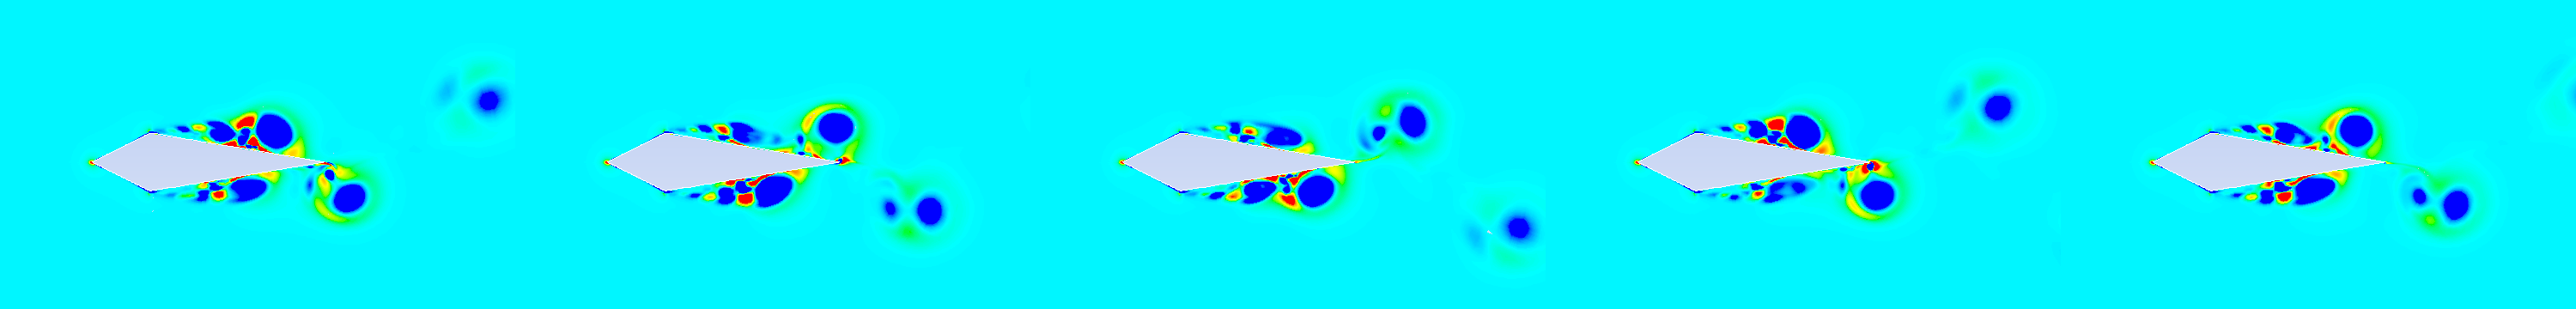
\includegraphics[height=0.8in]{./images/teaser.png}
  \caption{The vortex shedding pattern of flow over a 2D sword determines its dipole characteristics and the aerodynamic sound when swung by, say, a virtual samurai.}
}

\maketitle

\begin{abstract}

In this project, I explored the problem of real-time, physics-based aerodynamic sound synthesis for slender objects. It is largely inspired by the paper by Dobashi \etal~\cite{dobashi2003}. The aerodynamic sound when we swing a slender object, such as a stick, is originated from the complex interaction between the air flow and the stick. Sufficient spatial/temporal resolution was regarded to be essential to capture the physics and thus the characteristics of the sound generated. However, the required fluid simulation is too expensive to run at audio stepping rate. To avoid such computation, I first precomputed a comprehensive database that contains relevant sound textures evaluated from high-quality grid-based fluid simulation, and then at runtime, this database is fetched and textures are blended to effectively resynthesize the aerodynamic swinging sound. Next, to increase the interactivity of the project, I interfaced the sound system with Leap Motion sensor to give real-time motion capture data. The system is proven to be quite reliable and can run at real-time even on a low-end laptop, and create realistic swinging sound. 

\end{abstract}

%  \begin{CRcatlist}
%    \CRcat{I.3.3}{Computer Graphics}{Real}{Display Algorithms}
%    \CRcat{I.3.7}{Computer Graphics}{Three-Dimensional Graphics and Realism}{Radiosity};
%  \end{CRcatlist}

\keywordlist

%% Required for all content. 

\copyrightspace


\section{Introduction} 

In games and virtual environments, accurately representing the sound of moving a slender object quickly, such as a character swinging a club, is important for story telling and the realism of the environment. However, most of the time, this sound is faked by either playing back experimentally recorded ``canned'' sound, or by using random parametric models. These models are cheap to evaluate, but they lack physical basis of how the sound is generated, and therefore can cause noticable audio-visual synchorinzation problem or need a lot of hand-tuning to ensure the quality. Dobashi \cite{dobashi2003} presented the first automated, physically-based aerodynamic sound synthesis pipeline.

This class of aerodynamic sound is generated by the fluid flow around the object, and can be described by Curle's model \cite{howe2002}. Given two critical assumptions: (1) the object is acoustically compact, and (2) the listener is placed at a far-field position, the aerodynamic sound can be approximated by a dipole source, whose magnitude is governed by the unsteady forces generated by the object placed in the flow field. Section \ref{section:curle} specifies more details on this model.

Using this model, we computed fluid flow around the object of interest and the dipole sound source function, and cached them in a database for that object for runtime evaluation. At runtime, the propagation is modeled by use of free-space Green's function, and the sound source function was used to evaluate the sound at listener's position given the motion of object. Amplitude scaling based on Curle's model and frequency scaling based on Strouhal number were implemented. Section \ref{section:sound_texture} and Section \ref{section:runtime} discuss these parts. 

Leap Motion was configured to give a run-time motion capture data, and used as the input of our sound system. The basics of this interface will be described and demonstrated in Section \ref{section:runtime}. 



\section{Related Work} 

Fluid simulation has been used in the computer graphics community in realistic rendering of smoke, water, fire, and viscous fluid \cite{bridson_book}. However, most of the work has focused on creating compelling visuals rather than audio content. A few fluid sound projects can be found: bubble sound synthesis was explored by making use of a particle-based model to augment existing incompressible fluid solvers \cite{zheng2009}. The Minnaert model was used to mimic acoustical properties of bubbles \cite{vandenDoel2005}, and later extended to complement the use of fluid solvers \cite{moss2010}. However, the underlying physical principles of bubble sound generation are very different than those for aeolian sound. Bubble sounds are generated via individual or collective bubble oscillations, while aeolian tones are generated from the dynamical structure of vortices in the flow. Furthermore, numerical errors affect the bubble sound indirectly by altering its shape, whereas errors affect aeolian sound directly. Our approach make use of high-accuracy, mesh-based methods to minimize these errors.

Other physics-based sound synthesis work can be found for applications such as rigid-body motions \cite{obrien2002,vandenDoel2001}, thin shells \cite{chadwick2009}, and fractured materials \cite{zheng2010,chadwick2012}. However, these sounds are in principle generated by vibrating solids. The aerodynamic sound is generated by the oscillations of pressure field given a geometry. 

Sound texture modeling and synthesis methods can be used to resynthesize an audio corpus. Chadwick \etal~synthesized fire sound using a low frequency signal generated by physics-based simulation and then procedually added high-frequency content by means of bandwidth extension \cite{chadwick2011}. An \etal~used cloth simulation at graphics rates to drive a parametric model for both crumpling and friction events, and then applied a concatenative sound synthesis technique to map all features computed using the mel-frequency cepstral coefficients (MFCCs) to a experimentally constructed database \cite{an2012}. Other texture synthesis techniques such as inverse-FFT synthesis \cite{rodet1992}, and additive and subtractive synthesis also exist \cite{serra1990}. Verron \etal~built an additive synthesizer for environmental sounds, including wind sound \cite{verronphd}. This model was based on an additive synthesis method, which performs analysis on an input signal to obtain a spectral envelope and a set of parameters to reconstruct the sound or, by tuning the parameters, synthesize a new sound. 

Dobashi \etal~presented a precomputation method to synthesize aerodynamic sound that is the most similar to our approach. They made use of computational fluid dynamics to sample fluid flows over a slender object to create a soundbank of aeolian sounds (``swoosh'')\footnote{This paper showed a cavity tone demo, but contains no details of how it was done. The main focus of it was to simulate the swooshing sound.}, and resynthesize it at runtime based on an approach similar to the wavetable synthesis \cite{vandenDoel2001}. This is the main paper I am implementing.


\section{Curle's Model}  \label{section:curle}

For acoustically compact object and far-field listener, the sound pressure is governed by the equation \cite{howe2002}
\begin{align}
    p(\mathbf{q}, t) &= \f{1}{4\pi c_0 r^2} (\mb{q} - \mb{o}) \cdot \mb{g}(t-\f{r}{c_0}), \\
    \mb{g}(t) &= \f{\p}{\p t}\mb{F}(t) dS.
\end{align}
$\mb{q}$ is the listener position, and $\mb{o}$ is the object center position. $c_0$ is the speed of sound, $r$ is the distance between listener and object center, and $\mb{F}$ is the aerodynamic forces of the object in the texture domain, precomputed in the fluid simulation. Given this model, we can statically sample and cache the function $\mb{g}$ at different inflow speed and directions for a given object, and only evaluate the sound propagation at runtime. The runtime cost would be a data-fetching process, and a few flops to decide the position and direction of the object with respect to the listener in order to scale the sound amplitude and time delay.


\section{Sound Texture Database Construction}  \label{section:sound_texture}

The sound source function, $\mb{g}$, can be precomputed in a fluid simulation. I used proprietary finite-volume solver Ansys Fluent to do the computation. The object being sampled was placed in a virtual wind tunnel and rotated with $5$ degree interval to sample the sound source function for every inflow direction. To shorten this preprocess, the following identities are used
\begin{itemize}
    \item [(1)] The amplitude of the dipole sound scales linearly with inflow speed in the log-space. That is, $|p_v| = (v/v_0)^\alpha |p_{v_0}|$. $\alpha=6$ is the coefficient Dobashi used, but I found that $\alpha \approx 2$ works better because the high coefficient gives too wide the dynamic range.
    \item [(2)] The frequency of the dipole sound scales linearly with inflow speed. The physical argument here is based on the Strouhal frequency, $St = f D/v$, where $St$ is the Strouhal number, $D$ is the diameter of the cylinder, and $f$ is the frequency. For a wide range of Reynold's number ($Re=100 \sim 1E6$), the Strouhal number stays roughly constant for cylinder ($St_{cylinder} \sim 0.21$) and therefore for the same object, the frequency scales linearly with inflow velocity. Linear interpolation was applied to sound textures to first upsample it to avoid artifacts when we scale the textures. 
    \item [(3)] For inflow with non-zero incidence angle, the sound is approximately equal to the sound created by inflow speed scaled by the geometric factor. Therefore, all the inflow directions at runtime were projected to the normal direction of the object before the sound source function was evaluated. 
\begin{align}
    sound(v_\theta) \approx  sound(v_{\|}), \quad v_{\|} = v \cos\theta. \label{eq:incidence}
\end{align}

\end{itemize}


\section{Runtime Considerations} \label{section:runtime}



\subsection{Real-time motion capture}

Position, speed, and orientation of the object are the metrics needed to compute the aerodynamic sound. To test the system, I first drove the sound model using mouse cursor (only speed was used), and then I configured Leap Motion to obtain the position, speed, and orientation information in real-time. Intertextural blending is introduced at the second stage.  


\paragraph{Using mouse cursor} To drive the sound model using mouse, the cursor position in screen space was queried at every audio callback, and the speed of the cursor was computed using first-order explicity Euler method. No orientation effect was introduced at this stage (therefore only one texture was considered). 


\paragraph{Using Leap Motion} Next, I sought for low latency, stable sensors to compute runtime object orientation. I have tried Nintendo Wii's controller but the bluetooth interface was not stable, and the field-of-view (FOV) of its infrared sensor was too small to resolve swinging motion. I then found Leap Motion, which is a low-cost commerical sensor released in 2013. The mature API makes it quite easy to use. The Leap Motion system recognizes and tracks hands, fingers and finger-like tools. The device operates in an intimate proximity with high precision and tracking frame rate (on my machine the peak sampling rate can reach $150$Hz when lighting condition is good) and reports discrete positions, gestures, and motion. The Leap Motion controller uses optical sensors and infrared light. The sensors have FOV of about 150 degrees, making it a good candidate for the swinging application. Please see Fig.~\ref{fig:leapmotion} for more detailed description of this system.

\begin{figure}[ht]
  \centering
  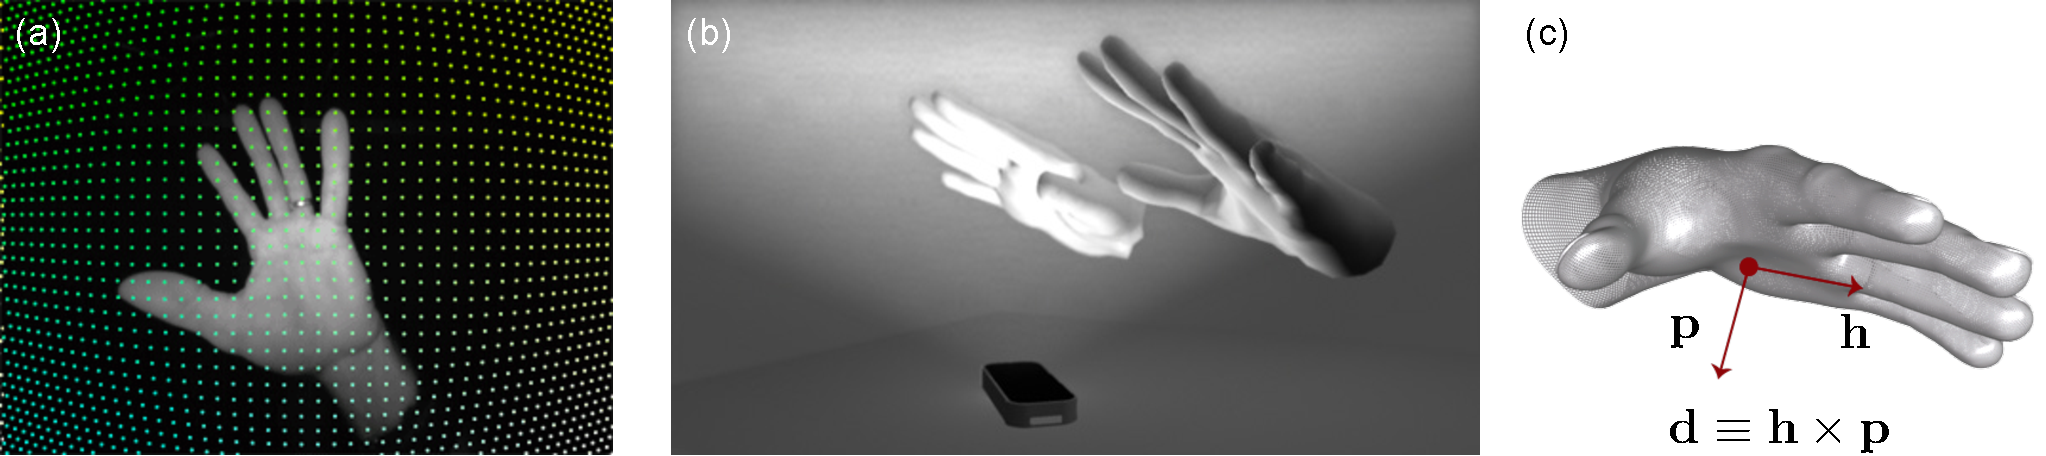
\includegraphics[width=3.5in]{images/leapmotion.pdf}
  \caption{Leap Motion sensor: (a) The system use IR sensors to detect the motion and gestures of the hand. The raw IR images can be used for debugging; (b) The system features a 150 degree FOV, making it a good candidate for our swinging motion; (c) The orientation of the object can be uniquely determined by transforming the wind vector into the coordinate system defined by the direction of the hand and the palm normal.}
  \label{fig:leapmotion}
\end{figure}

Knowing the direction of the hand, $\mathbf{h}$, and the normal direction of the palm, $\mathbf{p}$, the relative wind direction in the world space can be transformed to the object space. Using the identity for the slender object Eq.~\ref{eq:incidence}, the sound source function can then be fetched by projecting this wind direction onto the plane of the cross-section and quantized to an integer number that represents the index of the texture (5 degree interval for all cases). This process is illustrated in Fig.~\ref{fig:transform}. 

\begin{figure}[ht]
  \centering
  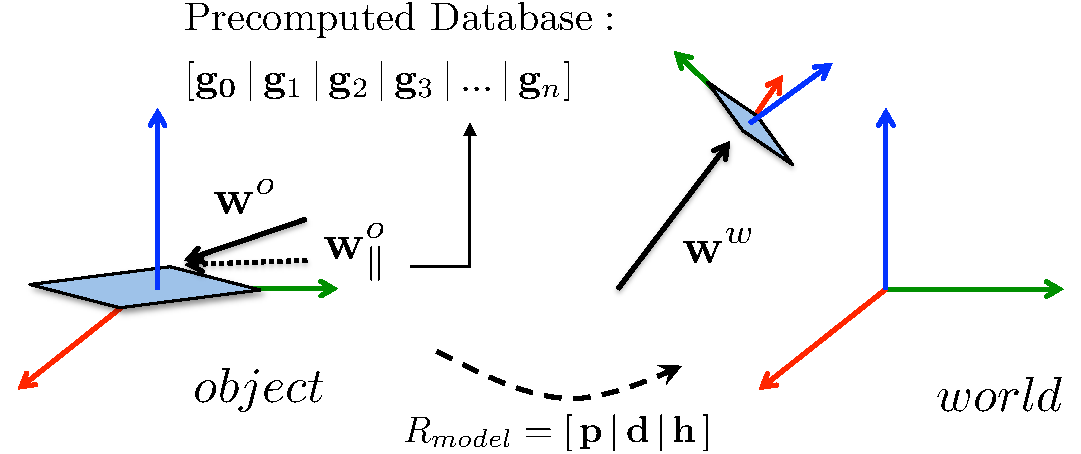
\includegraphics[width=3.0in]{images/transform.pdf}
  \caption{The wind direction, determined by the swinging motion, is first transformed into the object space, and then projected onto the plane of the cross-section. This vector, $\mathbf{w}^{o}_{\|}$, is then quantized into a texture index for this object to fetch the sound database, which is preloaded when the program starts.}
  \label{fig:transform}
\end{figure}

\subsection{Clicking noise and audio underrun}

One of the big problems I encountered when implementing this paper was how to do the real-time audio rendering properly, the discussion of which is missing from the paper. There were two main problems associated to it: (1) the time-scale mismatch in motion capture refresh rate and audio stream sampling rate can cause severe ``clicking'' sound when scaling the textures or jumping between textures. (2) the audio underrun caused by improper thread priority for audio callback and high motion capture latency.

The clicking problem (either caused by resampling the texture in the amplitude/frequency shifting or jumping between textures) can be resolved by requesting an optimum buffer size. To avoid audio glitch, the audio interface (I use portaudio) reduces the number of audio callbacks by requesting an audio buffer when the audio stream is opened. The size of the buffer can be fixed or adaptive, depending on the hardware implementation and the application (for example, the CoreAudio framework in MacOS is well written, and can largely reduce the latency). What I did to resolve the clicking was to enforce the motion-capture data to be sent only when audio callback happens, and then linearly blend between the two states of motion data (sound amplitude/frequency). I found that the buffer size of $\sim100$ works the best. If the buffer is too large, the motion-capture data is updated infrequenctly and the playback will sound sluggish; whereas if its too small, then the buffer doesn't have enough time to blend the textures and clicking will occur. Note that this number is roughly the ratio between audio sampling rate (for most of them is $10000$Hz) and motion-capture update refresh rate (at around $100$Hz).

The audio underrun happens when the buffer is not properly filled in the requested time frame, and portaudio has no choice but to substitute it with zeros. This problem can be severe if the implementation is not handling it explicitly. By requesting high-priority threads to the audio callback and to the motion-capture callback, the underrun problem can be alleviated if the space of sound source function for the object has reasonable size. Also, unbounded time operations such as file I/O should be completely avoided or minimized in the audio callback. For the same reason, the sound textures should all be loaded when the program starts, to avoid unnecessary underrun at the cost of higher memory footprint.


\section{Result} 

\subsection{Implementation Details} 

The project was implemented in C++. PortAudio\footnote{http://www.portaudio.com/} was used for audio control. Leap Motion API\footnote{https://developer.leapmotion.com} was used to control the device and interface with the sound system developed based on Dobashi's model. All the fluid simulation data was obtained using Ansys Fluent, a proprietary finite-volume solver. The simulation ran on 32 core desktop equipped with Intel Xeon processors. More statistics of the precomputation is given in Table \ref{table:runstats}. All the simulation geometry is given in Fig.~\ref{fig:simulation_geometry}. 

\begin{figure}[ht]
  \centering
  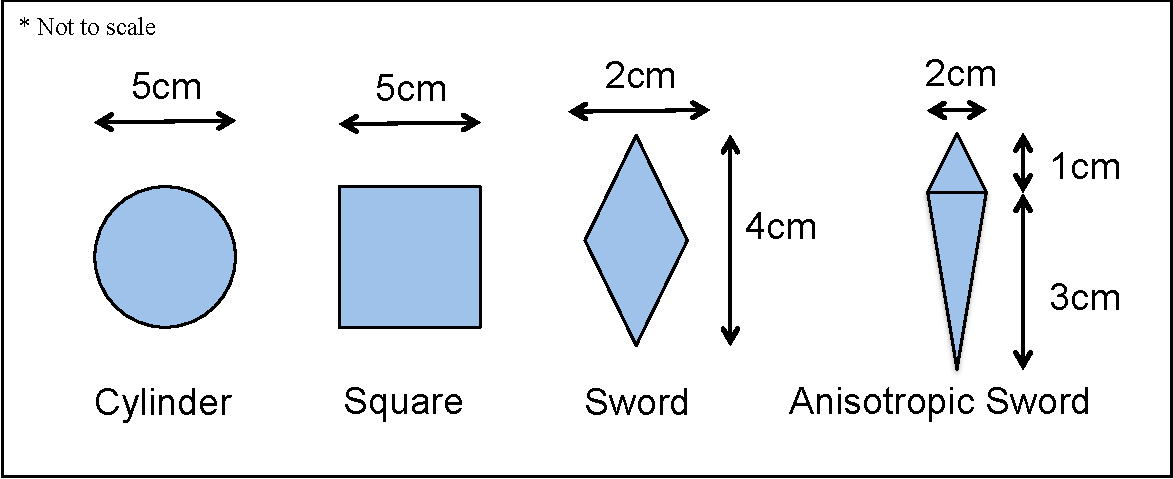
\includegraphics[width=3.0in]{images/simulation_geometry.pdf}
  \caption{Cross-section of the geometry used in the precomputation.}
  \label{fig:simulation_geometry}
\end{figure}

\begin{table*}[t]
  \centering
  \caption{Precomputation statistics.}
  \begin{tabular}{*{6}{c}}
    \hline
    \textbf{Shape} & \textbf{Dimension} & \textbf{Sampling resolution (deg)} & \textbf{\# Orientations} & \textbf{Cell number} & \textbf{Processing time / sample (mins)} \\
    \hline
    Cylinder & 2 & 5 & 1 & 18816 & 104.27 \\
    \hline
    Square & 2 & 5 & 10 & 42308 & 154.51 \\
    \hline
    Sword & 2 & 5 & 19 & 42308 & 123.46 \\
    \hline
    Anisotropic Sword & 2 & 5 & 37 & 31920 & 101.21 \\
    \hline
\end{tabular} \label{table:runstats}

\end{table*}

\subsection{UI design}
The UI interface includes an OpenGL window to render the instantaneous hand position, orientation, and speed for debugging purposes. There are options to toggle on/off options, for example frequency shift. Sliders are used to adjust sensitivity and amplitude scaling exponent at runtime to speed up the iterations. Demonstration please see Fig.~\ref{fig:UI}.

\begin{figure}[ht]
  \centering
  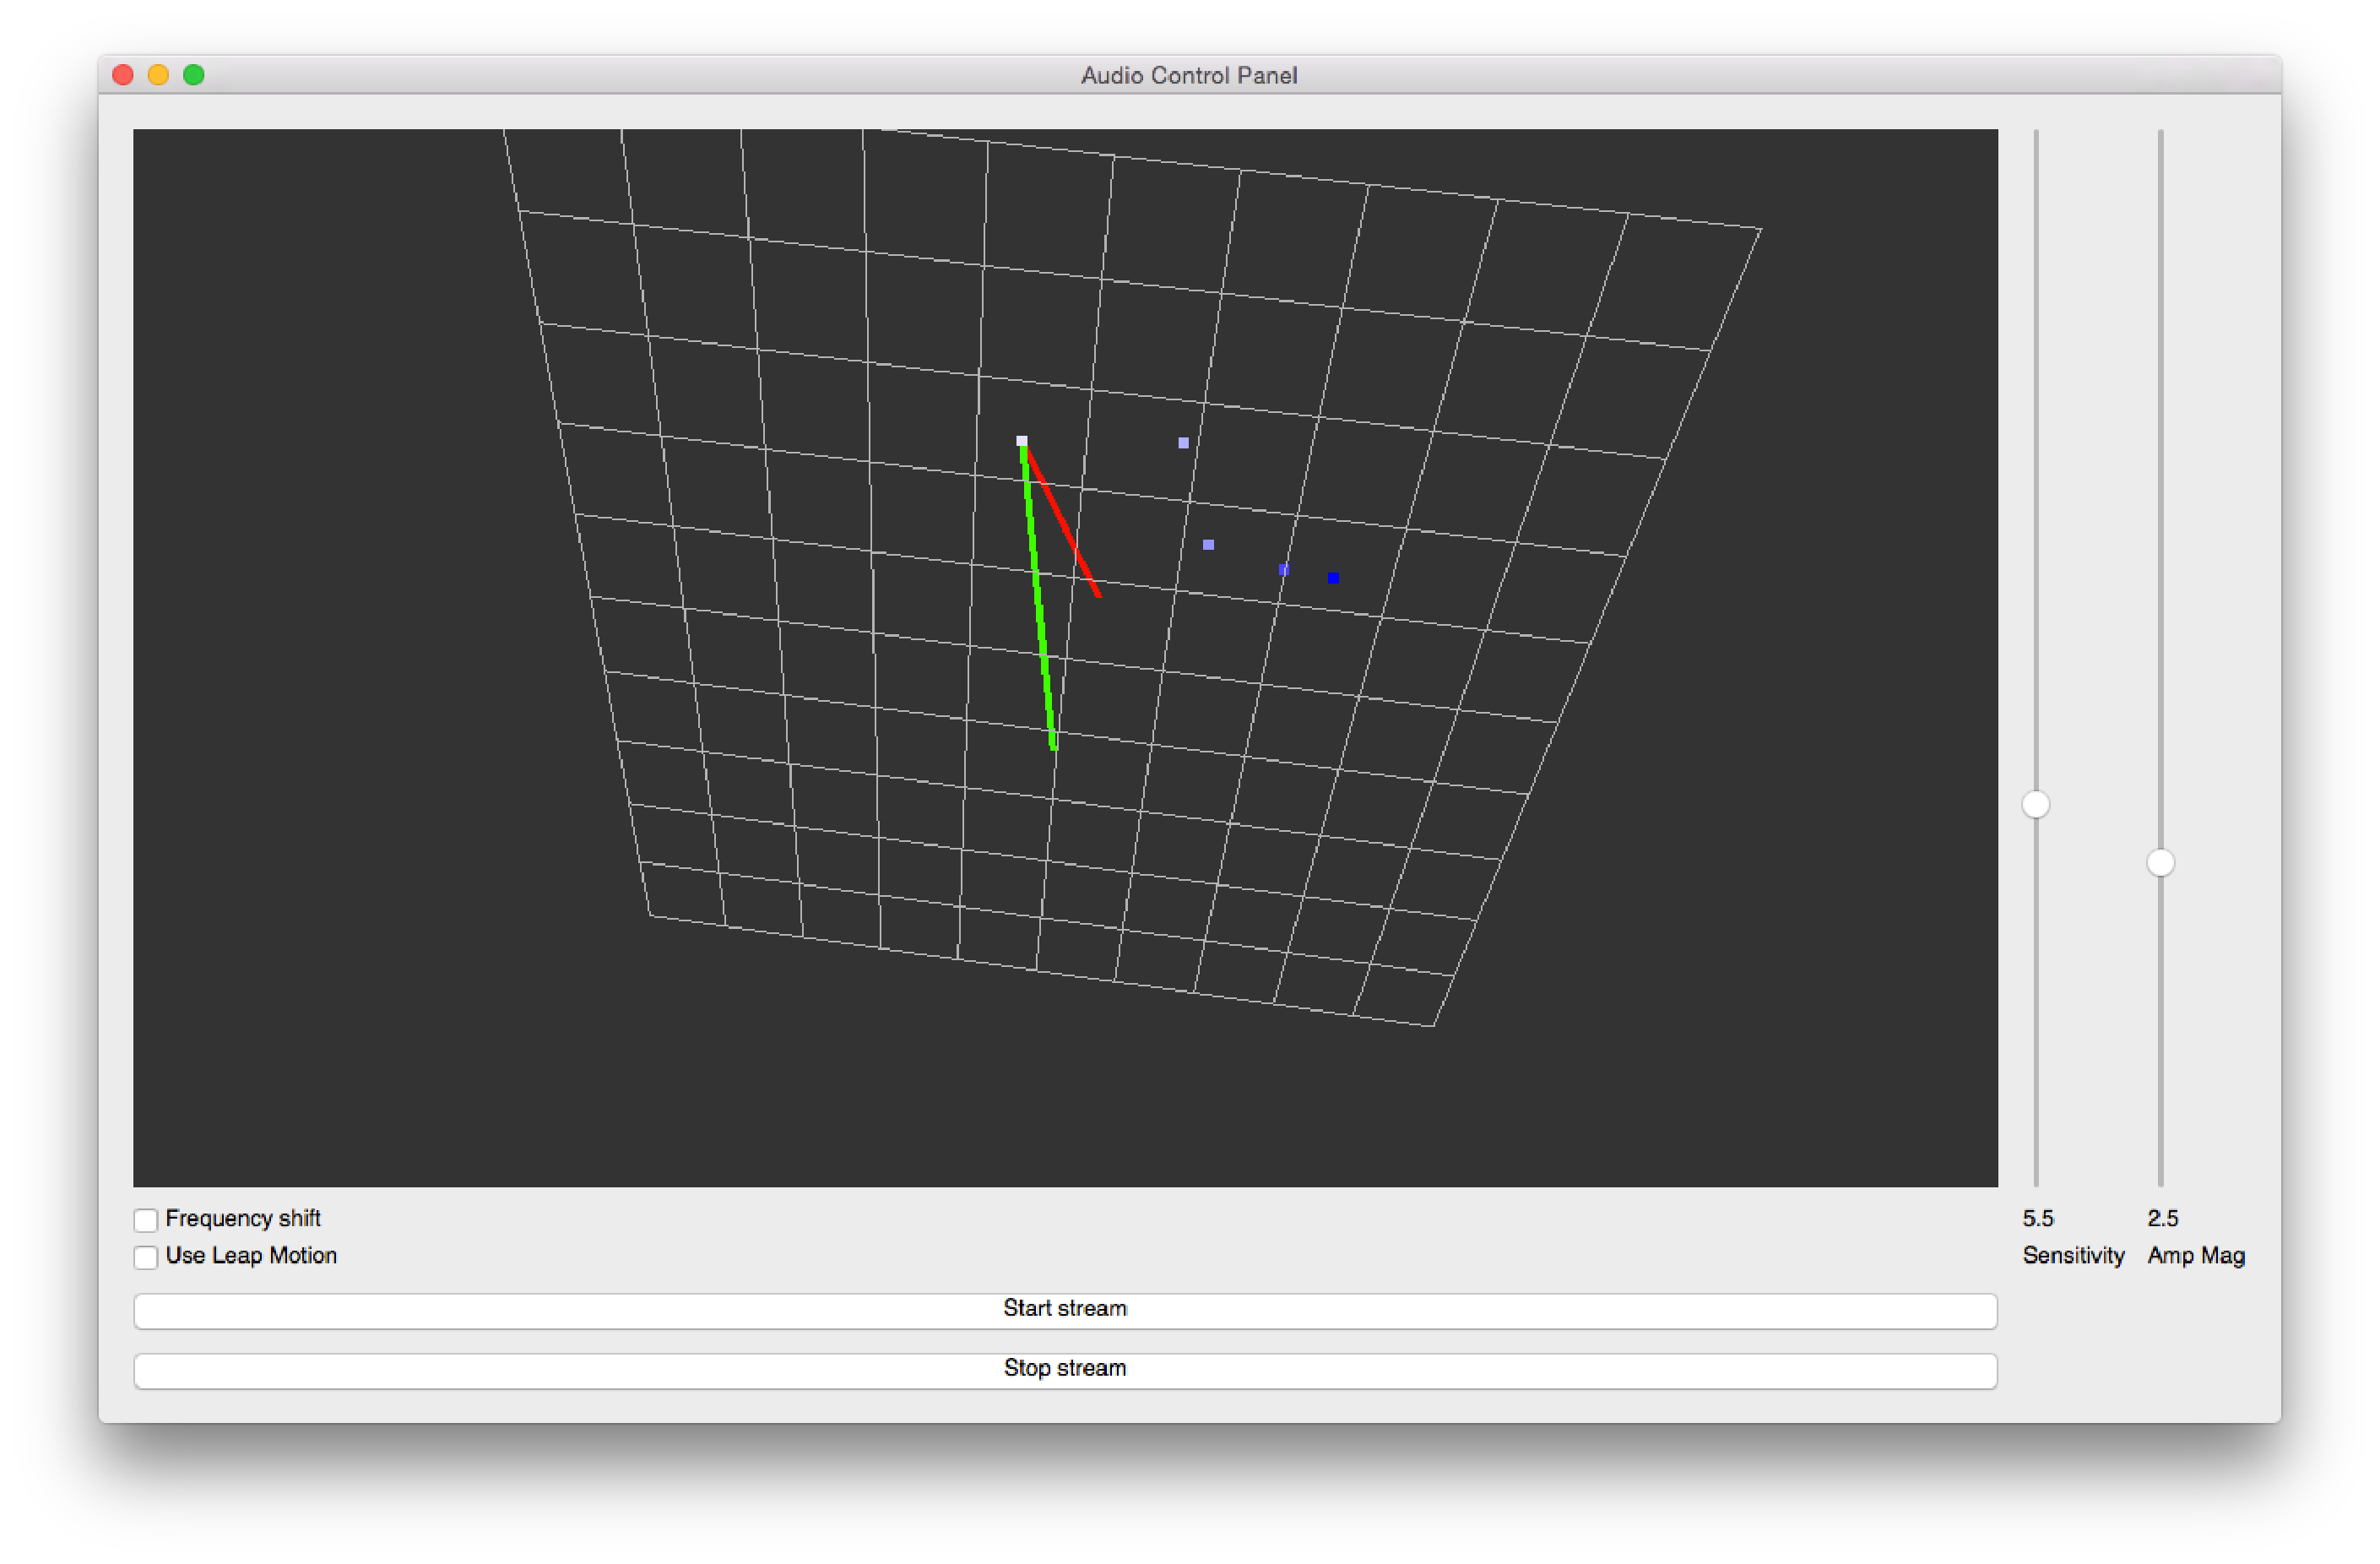
\includegraphics[width=3.0in]{images/UI.pdf}
  \caption{UI for the real-time control.}
  \label{fig:UI}
\end{figure}



\subsection{Motion capture data} 
My system run in real-time. However, for comparison purposes, one of the data sequence was recorded in order to use repeatedly to test different textures and geometries. One particular sequence was used throughout the rendering. The detailed tracking data for this sequence is shown in Fig.~\ref{fig:mocap}. Only the motion of the centroid of hand and tip of index finger are tracked in order to increase the frame rate as much as possible. From the figure, one can notice that the Leap Motion sensor is very reliable when palm direction is roughly aligned with table normal (that is, the silhouette is the clearest); however, when fingers are overlapped or palm is rotated, the tracking can be noisy.  

\begin{figure}[ht]
  \centering
  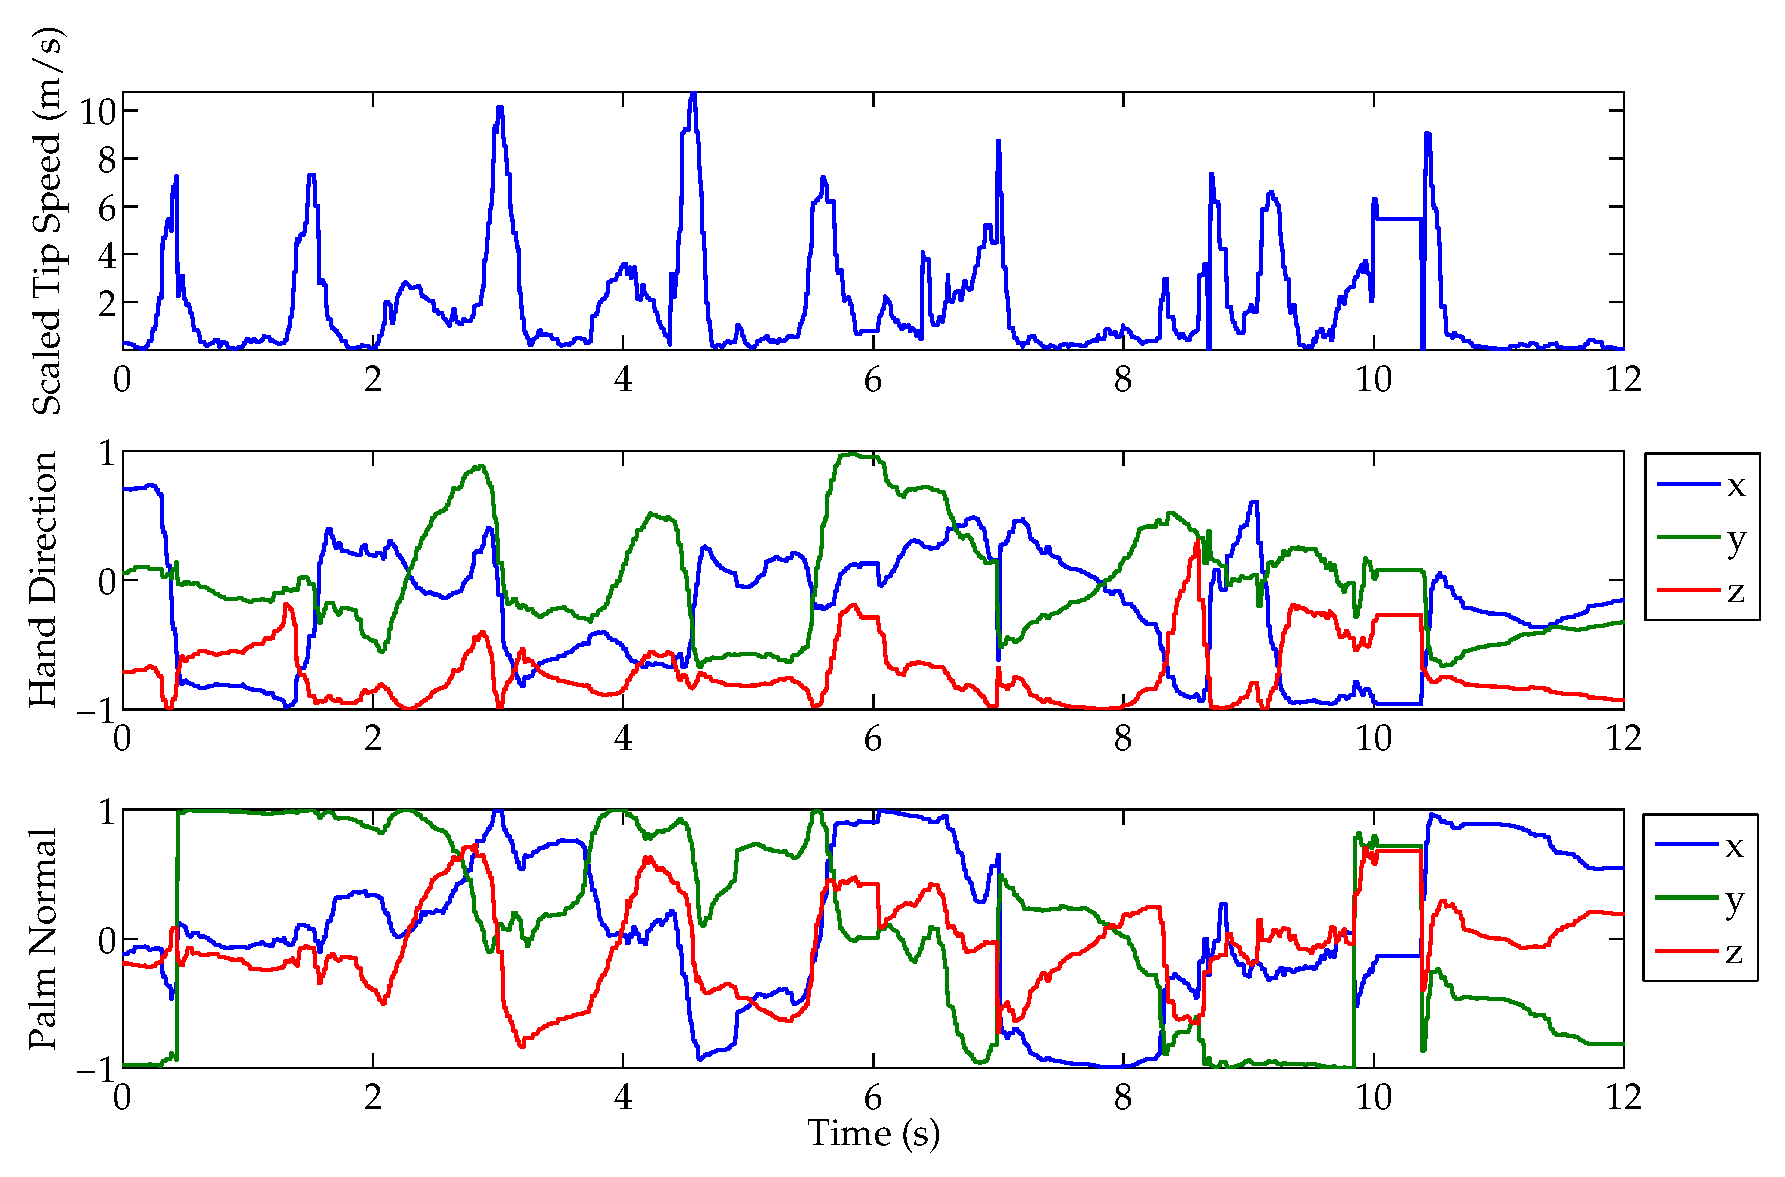
\includegraphics[width=3.0in]{images/mocap.eps}
  \caption{Example of motion capture data. Tip speed is scaled because my finger is too short to produce any interesting sound. X: point to my right when facing the computer monitor; Y: up direction; Z: towards me.}
  \label{fig:mocap}
\end{figure}

\subsection{2D cylinder} 
2D cylinder is the simplest case. Because of its symmetry, in total only 1 sample is needed if all three sampling properties are applied (introduced in Section \ref{section:sound_texture}). To validate the model, I ran a few more speed cases, and observe almost linear scaling in the peak frequency of the obtained sound clips (Fig.~\ref{fig:frequency_scaling}).

\begin{figure}[ht]
  \centering
  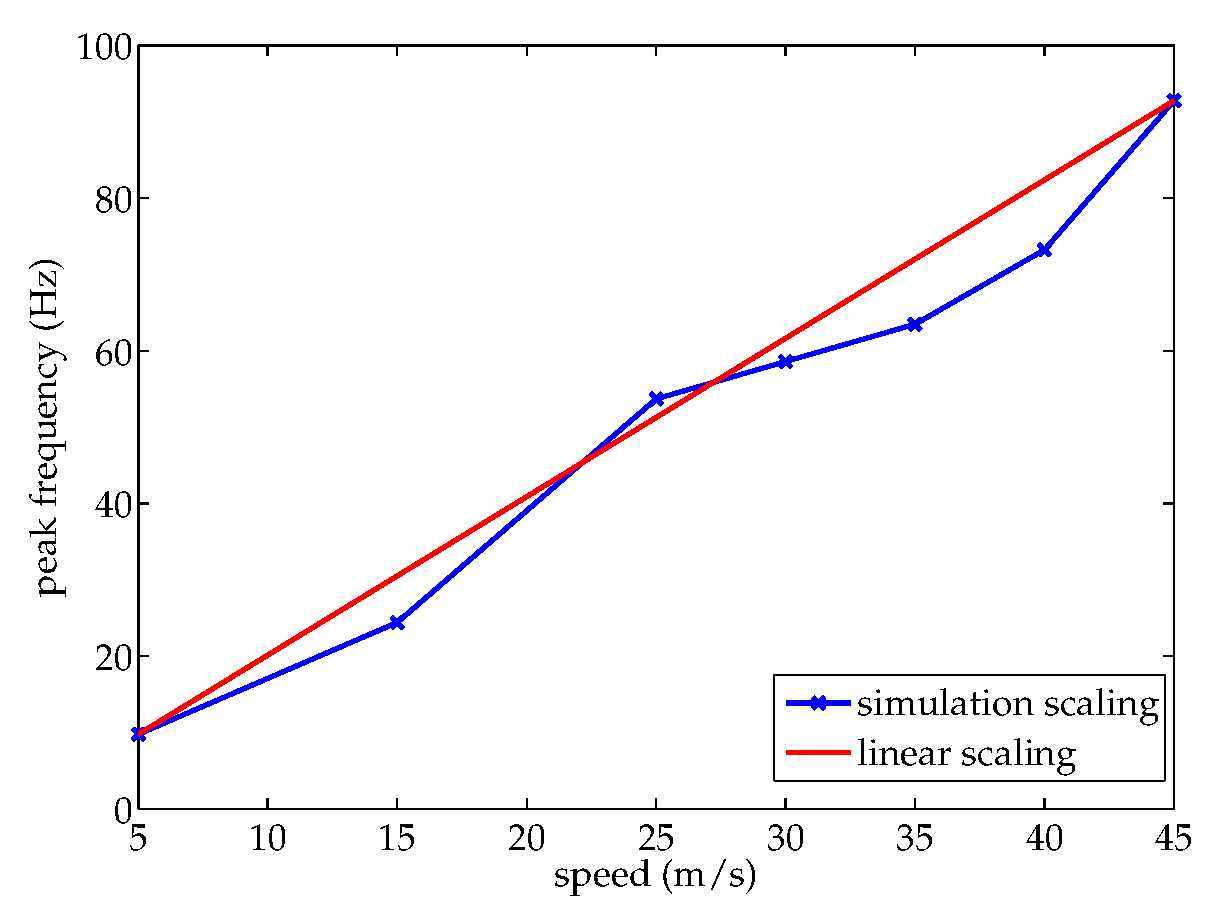
\includegraphics[width=3.0in]{images/cylinder_frequency_scaling.eps}
  \caption{The frequency scaling for cylinder introduced in Section \ref{section:sound_texture} is validated by running redundant speed sampling.}
  \label{fig:frequency_scaling}
\end{figure}

\subsection{2D square} 
2D square has certain rotational symmetry so the sampling only needs to cover 45 degrees. The sound changes only slightly when rotated but I observed increasing peak frequency (by only a little) when rotated away from the rest position shown in Fig.~\ref{fig:simulation_geometry}, potentially due to the increase of projected area.

\subsection{2D sword} 
2D sword needs to be sampled for 90 degrees in order to cover all its orientations. The geometry was recreated using the 2D square geometry case file and therefore the mesh count is the same in Table \ref{table:runstats}. The intertextural blending is also quite challenging since many textures need to be blended. What I did was to allocate a fraction of the audio buffer to first blend between textures, and then have the rest of the buffer used on blending single texture amplitude/frequency scaling.

\subsection{2D anisotropic sword} 
I spent the most simulation time on this test case. Unfortunately, the sampling for this object wasn't quite successful. The reason was because I changed a few simulation parameters for computing speed optimization but forgot to turned them back when it didn't work out. In the video, clear artifacts are audible when the sword is swung at certain angle. 



\section{Conclusion and Limitation}

I found the 6th power amplitude scaling does not work quite well because of the high dynamic range of amplitude variations, instead exponent of $2\sim3$ seems to work the best for my dataset. The linear frequency scaling was validated in additional simulation cases for cylinder geometry. Several geometries was sampled and compared using the same motion capture data (see video). Perceptually there is not a lot of interesting variation, but it could be due to (1) the motion-capture sequence did not properly excite the textures; (2) the geometries I picked were too similar in size such that the pitch shift (based on Strouhal scaling) is not obvious enough. Leap Motion sensor is great for its cost, however, the sampling rate and stability can be further improved using (the much more expensive) Vicon system, which can reach sampling rate of $1000$Hz; retroreflective markers would also help improving the tracking results instead of IR markers. 


This turned out to be a very fun project as I get to play with fluid simulation, real-time sound rendering, OpenGL, motion capture hardware and some aspects of parallel computing. I didn't have time to try the 3D object simulation, the description of which in the paper is actually quite unclear. In specific, how to discretize the 3D object and represent its force oscillations in different part was not mentioned at all. One alternative is to use the unsteady force for the entire object directly for each point source, but it is really hacky. Overall, I think this is a good paper given the difficulty of the problem and the computing capability back then, this method is cheap and can produce compelling results. 

% \section*{Acknowledgements}

\bibliographystyle{acmsiggraph}
% \nocite{*}
\bibliography{reference}
\end{document}


